\chapter{人脸多属性属性识别的架构}
本章主要介绍人脸属性识别任务数据库和一些人脸属性识别中常用的方法,并且根据这些方法的弱点和问题,提出改进方法改进并进行实验。包括人脸属性中输入图片对于识别效果的影响,改进网络结构对于属性性能的提升,设计面向多数据分布和多属性分类的神经网络框架、以及对于网络输出置信度模块的构建。

\section{人脸属性性质分析}
\subsection{人脸属性的类别}
人脸属性的数据标注的环境各有不同限制性场景和非限制性场景(如固定摄像头拍摄和日常采集的场景),其中标签往往具有很多种表示和性质,比如相对性标注和绝对属性标注(如颜值数据标注之间只有相互的高低,但没有绝对的属性标签)但总体分为有序性与无序性,整体性与局部性等,具体包括:
\begin{enumerate}
\item 无序性:
无序性的属性有两个或两个以上的类别(值),但在类别之间没有内在的顺序。 例如,种族是具有多个类别的名义属性,例如黑色,白色,亚洲等,并且这些值(类别)没有内在排序。;
\item 有序性:有序性的属性具有明确的变量排序。 例如,一个人的年龄,通常从0到100,是不平均的。(实际上,年龄不仅是相互独立的存在,在不同的年龄标签中,具有一定钟形的分布)
\item  整体性:
整体性标签描述了整个人脸的特征,诸如年龄,性别,种族等;
\item 局部性:
和整体性标签相反,局部性描述了部分人脸的特征,例如:尖鼻子,大嘴唇等。
\end{enumerate}
本文中也主要根据上面的人脸属性的性质来设计网络和分析问题。

\subsection{多属性标签表示形式}
在训练的过程中,人脸属性通常以分类或者回归问题的形式出现,但是在多属性识别的任务中,通常使用标签编码或者多标签回归的方式。

方法一:标签编码:
将多属性标签组合进行编码(比如,将一岁亚洲男性标记为001,将一岁非洲男性标记为002等),将多属性问题转化为分类编码问题,也就是单一属性。

方法二:多标签回归
通过回归的方法,使预测的特征向量与Groud-truth属性向量的损失越来越小,二者趋向接近,由此得到预测的特征向量。

\subsection{属性之间的相互联系}
正如上文提到的,属性之间具有非常大的异构性,但是作为人脸特征,它们同时在很多表现过程之中,也有很多共同的地方,那么在设计的过程中我们更倾向于用的是单框架多任务方式。这也利用属性之间的相关性,包括正相关和负相关等来进行互相补足;同时多任务的方式设计也应对属性之间的异质性,比如年龄是可量化的,而种族是类别化的,这就需要不同的处理方式。
我们对CelebA数据集的40个属性做了成对的co-occurrence计算,它揭示了,属性的相关性是普遍存在的,且我们认为它对属性学习有所帮助。
\begin{figure}[!ht]
 \centering
	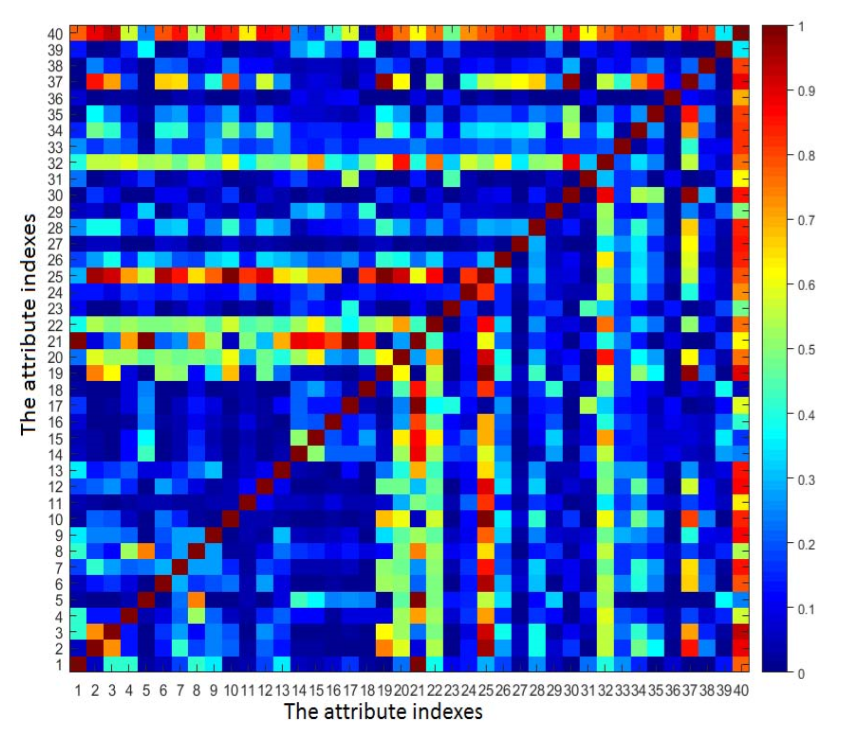
\includegraphics[width=6.0in]{attrconv.png}
	\caption{基于共享神经网络特征和SVM分类器的人脸属性识别}
\end{figure}

\section{人脸属性数据库简介}
这一章主要对于对于具体的数据库进行介绍:
\textbf{MOROH II:}MORPH是一个大型的mugshot图像数据库,每个数据库都有相关的元数据,包含三个标注属性:年龄(有序),性别(无序)和种族(无序)。通过调查MORPH Album II(MORPH II)上的所有三个属性估计任务,其中包含大约78K的超过20K个主题的图像。在MORPH II上的结果五等分数据进行交叉验证。

\textbf{CelebA:}CelebA是一个大型的人脸属性数据库拥有超过10万个身份的200K个名人图像,每个人拥有40个属性注释。该数据集中的图像在姿态,表情,种族,背景等方面存在较大的变化,使得面部属性估计具有挑战性。此外,由于有40个属性标注,CelebA数据库在特征学习效率方面对联合属性估计算法提出了挑战。

 \begin{table}
  \centering
   \caption{celeA中的属性表}
   \label{tab:req-pkg}
   \begin{tabular}{c|c|c|c}
     \toprule
     属性序号 & 属性 &属性序号 & 属性 \\
     \midrule
     |1|  & 5OClockShadow		 & |21| & GrayHair \\
     |2|  & Male 				 		 & |22| & Sideburns \\
     |3|  & ArchedEyebrows  	 & |23| & BigLips \\
     |4|  & MouthSlightlyOpen  & |24| & Smiling \\
     |5|  & BushyEyebrows  		 & |25| & BigNose \\
     |6|  & Mustache           & |26| & StraightHair \\
     |7|  & Attractive         & |27| & Blurry\\   
     |8|  & NarrowEyes 			 & |28| & WavyHair \\
     |9|  & BagsUnderEyes  		 & |29| & Chubby \\  
     |10| & NoBeard            & |30| & WearEarrings\\   
     |11| & Bald               & |31| & DoubleChin  \\
     |12| & OvalFace           & |32| & WearHat \\
     |13| & Bangs              & |33| & Eyeglasses \\
     |14| & PaleSkin           & |34| & WearLipstick \\
     |15| & BlackHair          & |35| & Goatee \\
     |16| & PointyNose         & |36| & WearNecklace \\
     |17| & BlondHair          & |37| & HeavyMakeup\\
     |18| & RecedingHairline 	 & |38| & WearNecktie\\
     |19| & BrownHair          & |39| & HighCheekbones\\
     |20| & RosyCheeks 			 & |40| & Young\\
     \bottomrule
   \end{tabular}
 \end{table}

\textbf{LFWA:}LFWA是另一个无约束的人脸属性数据库,其中包含来自LFW数据库的脸部图像(5,749个主题的13,233张图像),以及与CelebA数据库中相同的40个属性注释。

\textbf{Chalearn LAP and FotW:}ChaLearn挑战系列从2011年开始,在促进人们视觉或多模式分析方面取得了非常成功的成果。LAPAge2015是一个无约束的脸部数据库,用于在ICCV 2015上发布的视在年龄估计。该数据库包含4,699张脸部图像,每个平均年龄至少由10个不同的用户估算。数据库被分割为2,476张图像进行训练,1,136张图像进行验证,1,087张图像进行测试。由于年龄信息的测试不可用,主要使用validation集进行测试。 FotW数据库是通过收集来自互联网的公开可用图像创建的,其中包含两个数据集,一个用于辅助分类,另一个用于性别和微笑分类。 FotW数据集分别包含5,651,2,826和4,086幅用于训练,验证和测试的面部图像; 每个都用七个二进制附件属性注释(见表5(a))。 FotW性别和笑容数据集分别由6171个,3086个和8505个面部图像组成,用于训练,验证和测试; 每个都注明三元性别(男性,女性,不确定)和二元微笑的属性。 我们遵循相同的测试协议在FotW上报告结果。

这些数据库可以根据所使用的注释方法分为三类:(i)具有名义和有序属性的数据库(MORPH II和LFW +),(ii)具有二进制属性的数据库(CelebA,LFWA和FWW)和(iii) 具有单个属性的数据库(LAPAge2015)。 我们可以看到,除了MORPH II数据库,其他数据库主要包含真实场景下的人脸图像。  

\section{基于传统特征的人脸属性识别}
基于传统特征的人脸属性识别往往采用特征提取和分类器结合的方式,其中较为经典的是基于DIF特征的人脸属性识别是经典的属性学习方法,在morphII上一度取得了非常优秀的实验结果,基本框架概述如下:

前端为特征提取阶段,旨在提取对属性有判别力的特征,而不是完全无监督的。后端连接一个层级式的分类器,用于属性学习。具体结构见下图:
\begin{figure}[!ht]
 \centering
	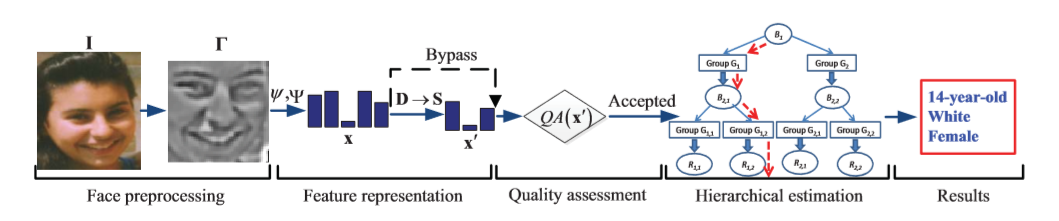
\includegraphics[width=6.0in]{huhanSTLMorph.png}
	\caption{基于DIF特征的人脸属性识别}
\end{figure}

其中有几个主要部分:DIF(Demographic informative features)特征提取,层级式分类器,人机对于单属性预测任务的对比

1)DIF特征:

DIF(Demographic informative features)是基于BIF(生物启发式特征)的。
比如,输入一个人脸部件,先用Gabor滤波器提特征(12个尺度,8个方向),再做一些池化操作,以减小特征图的数目和维度(6个尺度,8个方向),将得到的特征串成一个4280维的长向量,用来做之后的分类等任务。总体上还是一个无监督的特征处理方法。所以之后,又对此工作做了改进,旨在不仅能够抓住图像细节,还能减小冗余性,提高特征与最终识别任务的相关性。这一部分主要引入一些特征学习工作,从之前的特征集中不断特征子集,挑选出最相关的特征,比如:学习一个新的特征子空间(如LDA),基于Boosting的特征选择。

2)层级分类器的建设:

层级分类器主要针对年龄。比如,首先进行年龄组分类(针对数据集设定阈值),在此按是否超过18岁分为两类;低于18岁的一类再判断是否低于7岁,再分为两类,然后低于7岁再进行回归得到具体的年龄数值,以此类推,先一层一层地通过多个分类器树形展开得到具体的人脸年龄段,然后在具体的人连年龄分段中及进行回归。hu的实验证明,这种层级式的分类方式要优于直接分类方法。

基于DIF特征的属性识别方法是经典的基于传统特征和分类器的属性识别方法,即使在现在,特征融合、层级分类器建设等操作依然具有一定的借鉴意义

问题与不足:但存在一定的问题,例如,层级分类器确实能够提升分类的效果,但是复杂都明显过高,并不简洁,使用基于传统滤波器和表层信息的图像特征,需要大量的特征筛选和过滤工作。而且总结来讲是DIF系统还处在各个部分的分开设计,整个系统并不是处在一个整体性学习的状态。需要较多的人工干预和训练才能得到较好的效果。

\subsection{基于共享神经网络特征和最大间隔分类器的人脸属性识别}
随着深度学习方法的提出,深度学习的特征慢慢取代了传统的手工设计的特征,结合深度学习中经常使用的分类器,得到了更高的效果。
具有代表性的是基于级联CNN网络和SVM分类器的识别方法,使用两个CNN框架Lnet和Anet进行级联学习,其中Lnet负责检测图片中的人脸,Anet针对于Lnet中检测人脸使用交叉熵loss进行训练,为了提升识别的准确性使用SVM对于ANet中的特征进行训练。最后由SVM分类器输出具体的人脸属性预测值。
其中不难发现器图片的标签就采用的是标签化编码的方式。
\begin{figure}[!ht]
 \centering
	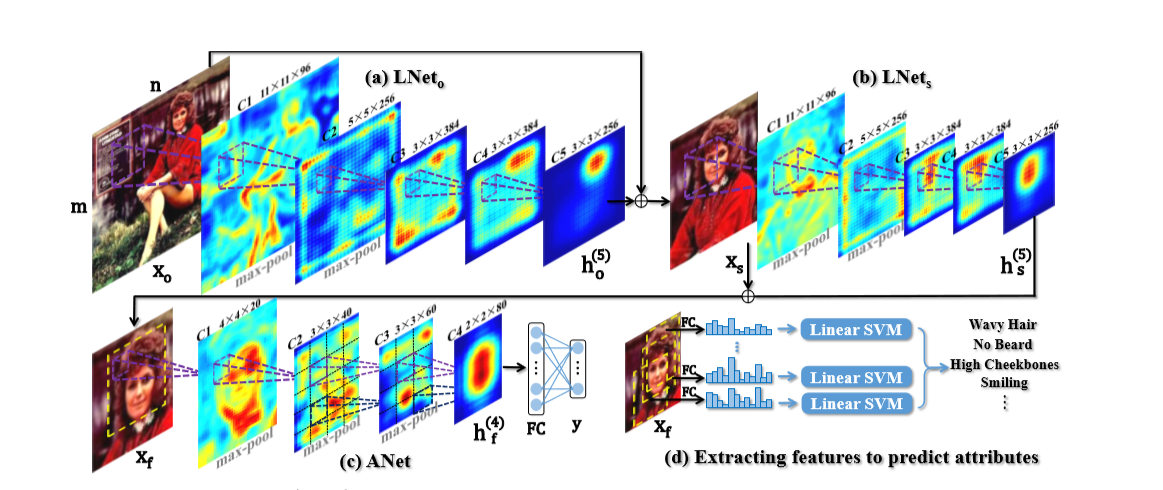
\includegraphics[width=6.0in]{liuziwei.png}
	\caption{基于共享神经网络特征和SVM分类器的人脸属性识别}
\end{figure}

问题与不足:其实在训练的过程中,神经网络就已经可以对于属性进行预测,但是识别的效果却并不如SVM训练的结果,说明在这一框架中,神经网络对于不同属性的自网络决策层和loss函数设计的不够好。从图中可以看到,不同的人脸属性之间都是用的同样的FC层全连接而来的。不能够体现出属性整体和局部特性。
 
\subsection{端到端的人脸属性学习}
机器学习神经网络中的端到端,一般是这指输入原始数据,输出最后结果的过程。




\begin{figure}[!ht]
 \centering
	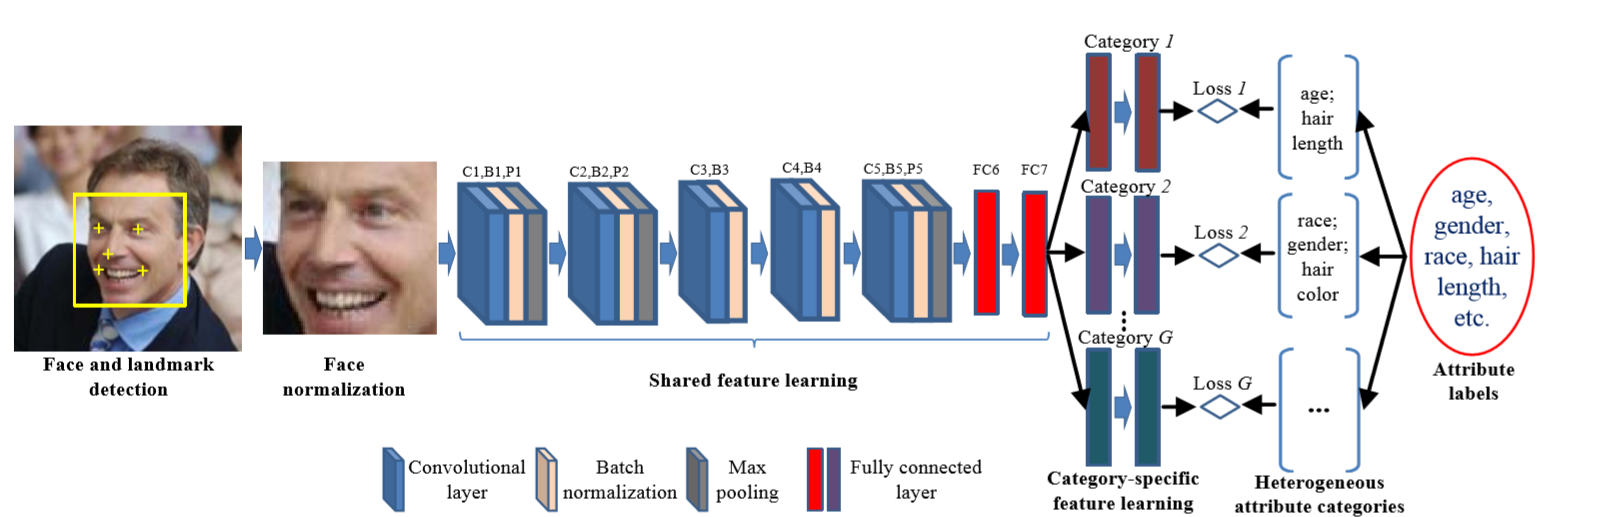
\includegraphics[width=6.0in]{huhanMTL.png}
	\caption{基于端到的人脸属性学习}
\end{figure}
 


\section{对于不同标注数据集中人脸数据的充分利用}
上面的两个工作其实已经解决了神经网络对于人脸属性的多任务学习问题,但是他们都有一个共同的缺点那就是,对于人脸数据的利用程度还不够,例如,虽然在各个数据集上Hu都进行了一定的评测,但是很明显,不同数据集的结果互相之间具有很大的差距,使用celeA训练的数据对于lfwA的数据效果并不好,实际上加入lfwA的数据训练就可以提升相关lfwA上的准确率。但需要注意的是LFWA的数据量远小于celeA的数据量,合起来训练,两个数据库之前的差异分布其实并不能得到特别好的弥补,训练的准确率还是不能和单独使用lfwA相比。
类似的问题更严峻一点,对于年龄这一属性,不同的数据库标注是不一样的,在morph中是连续的标签,但是在adience数据集上,年龄的标注是7个单独的类别,如果强行进行label的转换就会存在很多不匹配的现象,无法对其进行测试,但根据adience重新finetune,那么就会存在类似的数据匹配和模型输出改变的问题。
为了解决这一问题,我打破思维的限制,数据集并行训练的方式来解决这一问题,对于不同的数据集来讲,预处理的方式往往类似,也就是说输入图片虽然不同,但是输入的格式是一致的(事实上即使不同也没有什么问题,关键是图片数据不同),但是因为标签不同,导致在一个网络结构中无法进行统一的训练。那么不妨就按照多个单独的网络对于图像进行训练,每个网络在特征提取阶段采用相同参数的全卷及网络结构进行特征提取,但每一层的特征图会单独进行存储,训练的时候每个数据集都按照自己的数据结构特性为了拟合loss层的设计,采用不同的子网络结构。



\section{人脸属性识别中的网络能力自评估模块的设计}
这一部分主要希望讨论个人关于关于神经网络模式识别模型的评估的一些想法,在实验室的环境下,评价一个模型的好坏,一般的方法是测试他在公开测试集上的准确率;在实际的工程开发过程之中,评价模型的方法往往是现实的视频图片中的使用效果;但科学实验就是需要数值化的测试方法,并且人们相信至少我们先想办法吧准确率提高上去,这样以后面对新的困难,即使采用蚕食的方式也可以有类似的方式克服困难。这个想法激励着整个cv界的科研人员,也造成了CV界看上去是一个靠数据集吃饭的状态。学术界针对于数据集进行准 确率的提升和算法的改进和思考,工业界将相关的算法应用到实际的场景之中,进行不断优化以及寻找使用场景创造社会价值这就是整个计算机人工智能行业良好发展的一个重要原因。

事实上如果实验室评测的公开数据集能够很好的代表实际中所使用的数据,那么实验室的测试结果和现实的使用结果才可以具有相同比较意义,很遗憾即使是千万级的图像数据集也不能够完全代表和预测现实场景中所会遇到的问题,而实验室中过多的图片训练,也往往意味着需要参数更加复杂的模型进行训练,不仅对于训练的难度和实用性都提出了新的要求。在实际生产中类似的模型就会变得不可用,因为模式识别最基础的成本就是人工审核,如果机器预测的成本超过了人工成本,那么就没有使用机器预测的意义。

训练中模型评估:
在训练过程中,评估的指标有两种训练的loss和error,在训练的后期很多时候是模型的输出loss不断下降,但是error已经不再下降,所以

准确率不不应该是模型评测的唯一的评价标准,模型的稳定性同样是一个很重要的评价标准,也就是模型输出的方差。这一问题的集中体现表现在对于视频中的图形进行判断的过程中,视频输出的连续变化不要引起模型的巨变,比如对于同一个人在视频中不断调整姿态和动作,年龄模型的输出不应该随着这些产生特别大的波动。而模型产生波动的原因可能具体分析有很多,但总结的方法大概有两个,如果模型在自身的训练数据集同样没有达到特别好的效果,可能是因为模型的自身结构不够优秀;对于在训练数据表现出色的情况来讲,可能是模型训练数据不够全面。


测试中的模型评估:

加入背景类/模型自信度类别
改进softmax 

\section{实验设置}
再次回顾之前所提出的一系列问题:
1、

下面介绍神经网络中的单模型预测框架,得益于现代神经网络的出色表现,单属性预测模型的pipeline得到了极大的简化,同时结合端到端的设计思路和数据量的增加可以很好的提升单属性模型的预测效果。
CNN算法下的单模型输出预测:
首先经过图像预测处模块,将图像通过一些基础的图形变换转到统一的形变空间中,常见的操作包括图像识别任务中的空间颜色变换,尺度统一化,多尺度变换,多位置截取等。在人脸属性的人物之中,我们经常采用的方式是人脸alignment,也就是根据人脸检测输出的人脸边框位置和landmark,通过仿射变换,将人脸图像中的关键点映射到图像中的标准位置。

然后设计网络结构作为图像特征网络提取模块,这一部分往往有两条规则可以遵循从而有效的搭建神经网络结构,第一规则是根据现有的经典神经网络结构进行改进,比如alexnet,googlnet,resnet等,这样做有两方面考虑,一部分是因为这些网络在实际使用中“久经考验”,体现出了良好的收敛性能,另一方面由于类似的神经网络在科研的过程中使用的人数和场景比较多,在搭建和调参上会有很多共同的地方可以互相交流,也方便不同方法的比较。
所以总结来讲,其实如果主要的研究问题不在网络结构后对于识别任务的影响上,一般还是会使用业界通用的网络结构。
第二条规则就是在自己设计附加的网络结构过程中,也要符合一定的网络特性,包括结构上的自洽,设计之中不能产生模块之间不匹配的情况,比如同一层网络输入大小相互有差别,网络操作参数设置不合理等初级问题等,这一点看上去很简单,实际上出错的几率非常大。
针对于图像任务的标签选取不同的损失优化函数,常见针对于非连续的数据标签如分类问题,可以选取softmax cross entropy loss	的集合,亦可以针对于每个分类标签设置为多个二分类的问题,然后多个的二分类的标签联合训练使用交叉熵loss进行训练,当然这两种loss本身具有很多相似的地方,且在类别中只有两类的时候,具有相同的表达形式,但由于softmax with cross entropy loss的简洁形式,往往再多分类问题中选取这种损失函数。
我们也做了一些相关性的对比实验,发现整个模型的效果和时间都较之前有了很大的提升。
(插入图表 todo)

简单介绍一下人脸矫正的过程:

经过人脸矫正之后,不同的算法和模型其实是对人脸矫正之后的图片或者说一定3*H*W维数值分布在(0-255)的向量空间进行各种线性和非线性计算,最后输出图片对应的属性分类标签的过程。
(加一个简单的流程图)
人脸矫正顾名思义:就是将不够“端正”人脸调整到标准的大小,位置和姿态,这样可以让人脸都在同样的环境下进行比较,人的面部姿态一般会从roll(平面旋转), pitch(左右侧脸)和yaw(抬头低头)三个维度来描述。平面旋转很容易处理,只需将图片旋转一个角度调整至水平即可。而侧脸和低头处理起来比较有挑战,但通过放射变化也可以较好的解决。
在具体介绍人脸属性的任务过程中,首先对于人脸属性的一些常见问题做简单的介绍:
人脸属性识别的输入一般为具体的RGB图片,同时至少带有人脸检测输出的人脸框以及用于人脸矫正的landmark,实际实验证明,经过矫正的人脸对于和人脸姿势无关的属性具有很好的提升。

3)人机性能对比

人机性能比对是指和实际的人眼评估进行比较,这也是人脸识别领域中经常使用的指标。在人和机器的性能对比过程中,发现机器识别能力的绝对误差要小于人类。当在做年龄估计时,算法估计偏差比较平衡。而人类往往会将年龄估计偏高。但是机器会犯一些偏离实际较大的低级错误,这也是很多学习算法的共同问题。
